\Introduction

Важной задачей изучения аттракторов внутренних волн с помощью численных методов является обеспечение возможности проводить численные эксперименты с геометрией, приближенной к геометрии реального дна океана. Выполнение этой задачи ускорило и удешевило бы процесс непостредственного поиска аттракторов внутренних волн в океане, и изучение влияния аттркаторов на турбулентные режимы. Метод спектральных элементов, который обеспечивает достаточную точность воспроизведения результатов эксперимента, ограничен в своей реализации сложностью геометрии расчетной области. В свою очередь, метод конечного объема позволяет работать со сложной геометрией, которая способна имитировать поверхность океанического дна, но стандартные реализации не обладают достаточной точностью. Кроме того, монохроматический источника возмущений может не описывать реальные внешние воздействия. Зачастую, при моделировании явлений, связанных с образованием аттракторов в реальных условиях, необходимо учитывать несколько приливных воздействий \cite{Garrett1972} и изменение стратификации.

Явление внутренних волн представляется собой нарушение состояние равновесия на границе раздела водяных слоев различной плотности. Выеденные из равновесия частицы жидкости начинают совершать колебания под действием силы тяжести и силы Архимеда.

Считается установленным, что впервые внутренние волны наблюдал американский ученый Франклин в восемнадцатом веке с помощью простой экспериментальной установки. Она представляла собой емкость, заполненную несмешивающимися жидкостями различной полости~\cite{Sudolski}. Однако в конце восемнадцатого века вблизи полуострова Таймыр произошло событие, которое заострило внимание научного сообщества на этом интересном явлении. В то время в этом районе пролегал маршрут исследовательского судна <<Фрам>>(Рис. \ref{fig:fram}) под руководством Фритьофа Нансена (Рис. \ref{fig:Nansen}).

Однажды во время штиля судно остановилось. Скорость его движения резко снизилась.  «чтобы пройти то небольшое расстояние, которое мы и на веслах прошли бы в полчаса или того меньше, «Фраму» понадобилась целая вахта», -- как писал сам Нансен. При этом исследователь отмечал, что вода на поверхности была пресной, потому как натекла с оттаявших ледников. А на глубине сравнимой с осадкой судна, резко становилась соленой. Позднее его записи послужили стимулом для теоретических исследований этого явления. В итоге было установлено, что почти вся энергия судового двигателя сдвигает не судно, а образует волны на поверхности раздела между слоями пресной и соленой воды. Это явление получило название <<мертвая вода>>.

Также существует еще одно свидетельство этого явления. Теплоход «Маршал Жуков» при проходе пролива Дарданеллы угодил в <<мертвую воду>> летом 1981 года. Уже в сентябре в отраслевой газете <<черноморец>> капитан-наставник Александр Косилов подробно описал как в течении четырех суток судно, держащее курс из Канады в Новороссийск, боролось с феноменом. Согласно комментариям руководителя аналитико-исследовательской группы управления инвестиций и проектов ОАО «Новошип», кандидата технических наук, профессора кафедры судовождения ГМУ им. адмирала Ф.Ф. Ушакова Юрия Пескова современные суда в значительной степени подвержены влиянию подобных явлений\cite{MorVest}. На то есть причины:

\begin{itemize}
    \item Экономия топлива вынуждает снижать скоростные режимы
    \item Борьба за уменьшение углекислых выбросов предписывает снижать мощность двигателя
\end{itemize}


\begin{figure}
    \centering
    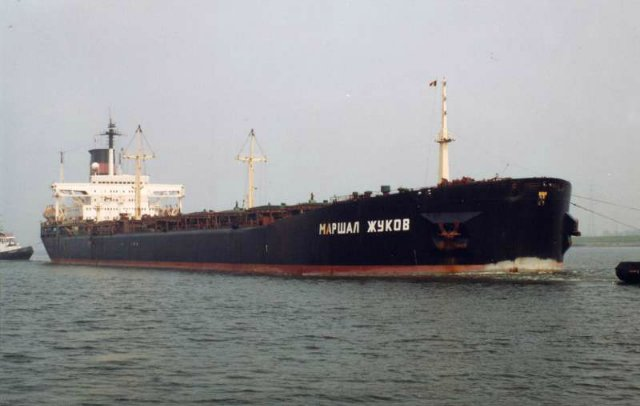
\includegraphics[scale=0.5]{Figs/marshl_jukov.jpg}
    \caption{Судно <<Маршал Жуков>>}
    \label{fig:jukov}
\end{figure}

И подобные явления, как оказалось, описывались и задолго до Франклина. В своей <<естественной истории>> Плиний Старший говорит о похожем явлении \cite{Plinii}. Позднее <<мертвая вода>> была воспроизведена в лабораторных условиях исследователями из франции \cite{deadWater}. Запись эксперимента доступна на видеохостинге youtube \cite{deadWaterVideo}.


Математически описать возникновение внутренних волн можно записав уравнение для сил, которые действуют на выведенную из равновесия частицу жидкости(Рис. \ref{fig:Forces}):

\begin{equation}
    m_b \vec{a}_b = \vec{P} + \vec{G}
\end{equation}
где $\vec{P}=\rho_w \vec{g} S \cdot h$ это сила Архимеда, $\rho_w$ плотность жидкости того слоя на котором находится частица, $\vec{g}$ -- ускорение свободного падения, $S$ -- площадь стороны частицы, $h$  -- глубина. $\vec{G} = \rho_b \vec{g} S \cdot h$,  $\rho_b$ -- плотность частицы жидкости.

В проекции на вертикальную ось:

\begin{equation}
    \frac{d^2 \xi}{dt^2} = \frac{(\rho_w-\rho_b)}{\rho_b}\cdot g
\end{equation}

Тут $\xi$ будет обозначать отклонение от положения равновесия $z_0$, тогда очевидно что плотность воды вокруг частицы и плотность частицы будет равна в положении равновесия при $\xi=0$ $\rho_w(z_0)=\rho_b$ тогда уравнение можно переписать:

\begin{equation}
    \frac{d^2 \xi}{dt^2} = \frac{\rho_w(z_0+\xi)-\rho_b}{\rho_b}\cdot g
    \label{eq:beg}
\end{equation}

Введем переобозначение, $z=z_0+\xi$ тогда правая часть уравнения запишется $$\frac{\rho_w(z_0+\xi)-\rho_b}{\rho_b}\cdot g = \frac{\rho_w(z)-\rho_w(z_0)}{\rho_w(z_0)}\cdot g = \frac{1}{\rho(z_0)} \frac{\rho_w(z)-\rho_w(z_0)}{z-z_0}\cdot(z-z_0) g$$

При достаточно малом $t$ отклонении от положения равновесия $z$ будет также мало, что дает нам возможность перейти к производной по $z$, а $\rho_w$ переобозначим как $\rho$ и окончательно запишем:

\begin{equation}
    \frac{d^2 \xi}{dt^2} =\frac{1}{\rho} \frac{d\rho}{z}\xi \cdot g
\end{equation}

Решение этого дифференциального уравнения ищется в виде периодической функции, это значит, что частица совершает колебания около своего положения равновесия:

\begin{equation}
    \xi(t)=A cos(\omega t + \phi)
\end{equation}

подставим выражения $\xi(t)$ в уравнение:

\begin{equation}
    \ddot{\xi} = - A \omega^2 cos(\omega t + \phi )
\end{equation}

или если выразить правую часть через $\xi$

\begin{equation}
    \ddot{\xi} = - \omega^2  \xi
    \label{eq:final}
\end{equation}

Подставим (\ref{eq:final}) в (\ref{eq:beg}):

\begin{equation}
    -\omega^2 \xi = \frac{1}{\rho_0}\cdot \frac{d \rho}{d z} \xi g
\end{equation}

Выразим частоту колебаний частицы:

\begin{equation}
    \omega(z) = N(z) = \sqrt{- \frac{g}{\rho_0}\cdot\frac{d \rho(z)}{dz}}
\end{equation}

Эта частота называется частота плавучести или Частота Брента — Вяйсяля. В океане она составляет величину порядка $10^{-3}$ $\frac{1}{\textup{с}}$ \cite{King2012}.

\begin{figure}
    \centering
    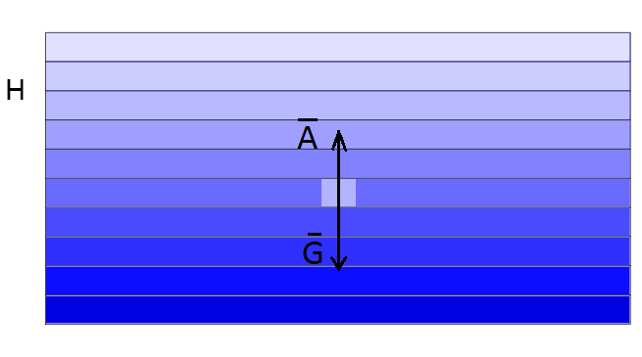
\includegraphics[scale=0.8]{Figs/Forces.png}
    \caption{Схематичное представление сил действующие на частицу выведенную из равновесия в стратифицированной жидкости, цветом показана плотность.}
    \label{fig:Forces}
\end{figure}

\begin{figure}
    \centering
    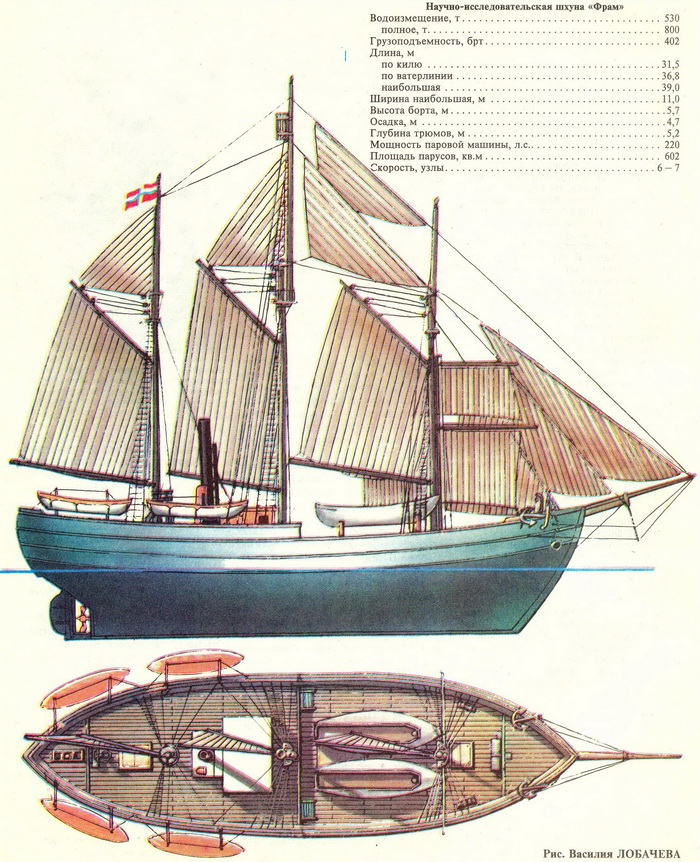
\includegraphics[width=1\textwidth]{Figs/FRAM.jpg}
    \caption{Исследовательское судно <<Фрам>>}
    \label{fig:fram}
\end{figure}

\begin{figure}
    \centering
    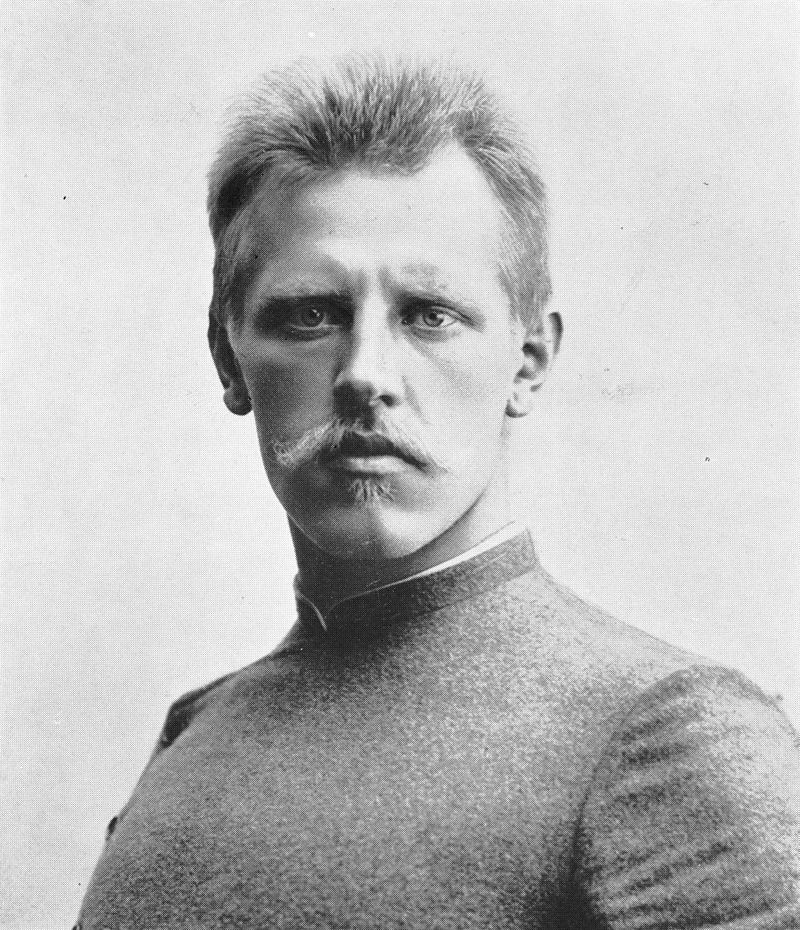
\includegraphics[scale=2.5]{Figs/800px-Fridtjof_Nansen.jpg}
    \caption{Фритьоф Ведель-Ярлсберг Нансен (1861-1930)}
    \label{fig:Nansen}
\end{figure}

\section{Обзор литературы}

Внутренние волны очень распространенное явление в океане. Существуют они благодаря перепадам плотности на разной глубине, сила плавучести играет роль восстанавливающей силы. Океаны являются одним из естественных примеров стратифицированных сред. Основные источники внутренних волн в океане это приливные эффекты, которые сопряжены с движением Земли относительно Солнца и Луны относительно Земли.

Внутренние волны активно взаимодействуют с другими океаническими структурами \cite{Rainville2006} и с неровностями океанического дна \cite{DAUXOIS1999}. Процессы перемещения внутренних волн их взаимодействия друг с другом и океаническими структурами различных масштабов образуют собой явление называемое энергетическим каскадом\cite{Garrett1972}. Энергетический каскад способствует поддержанию глобальной океанической циркуляции и перемешиванию\cite{Nikurashin2012,Munk1998}. Тем не менее, механизмы вносящие крупномасштабный приливный вклад в движение внутренних волн недостаточно понятны \cite{Ivey2008,Polzin1997} и каскадный процесс остается одной из фундаментальных проблем современной океанографии. Главным образом остаются вопросы связи крупномасштабных и мелкомасштабных явлений.

Одним из объяснений этой связи могут послужить аттракторы внутренних гравитационных волн. Это явление, при котором внутренние волны многократно отражаясь от поверхности океана, его дна и неровностей движутся по замкнутым орбитам. Возникновение такого явление возможно лишь в том случае, когда на дне океана имеются определенные комбинации геометрических неровностей. Аттракторы передают кинетическую энергию крупномасштабных эффектов, такие как приливы и внутренние волны большой длинны к мелкомасштабным явлениям волновой турбулентности и перемешиванию. Происходит это благодаря явлению фокусировки, в результате которого длинна внутренних волн уменьшается, но увеличивается амплитуда.

Возможность возникновения аттракторов в океане с реальной геометрией дна уже исследовалась\cite{Tang2010}. Например, топология северной части хребта Лусона имеет соответствующую геометрию. Эксперименты~\cite{ECHEVERRI2011} подтверждают возможность образования аттракторов внутренних волн. Кроме того при моделировании внутренних волн в условиях случайного разреза геометрии океанического дна, был сделан вывод, что с немалой вероятностью возможны возникновения аттракторов по одному на каждую сотню километров океанического дна \cite{Guo2015}. Тем не менее стоит отметить, что на данный момент нет свидетельств наблюдаемых волновых аттракторов. Возможно это связано с тем, что теоретические работы\cite{Guo2015} относятся к двумерному океану, но также существуют трехмерные конфигурации геометрий в которых возможны существования трехмерных волновых аттракторов\cite{Drijfhout2007,Manders2004}. Кроме того, в теоретическом представлении аттракторов внутренних волн не учитывается шероховатость поверхностей отражения. Однако надежность теоретических соображений о возможности существования трехмерных аттракторов была экспериментально проверена\cite{Hazewinkel2010}. Кроме того волновые явления в океане часто имеют целый спектр частот\cite{Garrett1972}, в то время как многочисленные эксперименты проводятся лишь с монохроматическим источником внутренних волн.

Предполагается, что аттракторы могут влиять не только на перемешивание, но и на движение мелких животных, явление седиментации и эрозию прибрежных конструкций.

Работы по фокусировке внутренних волн и образованию устойчивых аттракторов ведутся с конца двадцатого века. Первое теоретическое предсказание аттракторов было сделано Лео Маасом в 1995 году\cite{Maas1995}. Через два года последовали экспериментальные исследования этого явления, теоретические результаты были воспроизведены\cite{Maas1997}. Эффекты фокусировки характерны не только для стратифицированной жидкости, но и для вращающихся \cite{articleMaas2003,Veronis1970}. В дальнейшем теоретические основы явления были пересмотрены на основании данных эксперимента\cite{Lam2008}.

Вместе с развитием вычислительной техники развивались и инструменты численного моделирования физических явлений. Во втором десятилетии двадцать первого века стало возможным численное моделирование трехмерных аттракторов внутренних волн. Первая удачная попытка была предпринята с использованием метода спектральных элементов\cite{Brouzet2016,Brouzet_2016}. При сравнении с экспериментом ошибка численного моделирования составила не больше 10\%. Также была предпринята попытка моделирования аттрактора внутренних волн с помощью метода конечного объема\cite{Brouzet2014}. Количественно воспроизвести результаты, полученные с помощью метода спектральных элементов не удалось.
Традиционно для моделирования аттракторов применяются уравнения Навье-Стокса в приближении Буссинеска. Однако существует ряд работ, где вместо классического подхода используется квазигидродинамический\cite{ElizarBook}. Квазигидродинамические уравнения позволяют добиться большей точности\cite{Kraposhin20182} при моделировании методом конечного объема.


% В ходе работ был разработан программный продукт, который подлежал государственной регистрации № 2018663951.
